\hypertarget{cv:registrarMensaje}{\section{Registrar Mensaje}} \label{sec:registrarMensaje}

	Esta funcionalidad le permitirá registrar un término de glosario dentro del proyecto que se esta operando. 

		\subsection{Procedimiento}

			%Pasos de procedimiento
			\begin{enumerate}
	
			\item Oprima el botón \IURegistrar{} de la pantalla \ref{fig:GestionarMensajes} ''Gestionar Mensajes''.
			
			\item Se mostrará la pantalla \ref{fig:registrarMensaje} ''Registrar Mensaje''.

			%Pantalla
			\begin{figure}[H]
				\begin{center}
					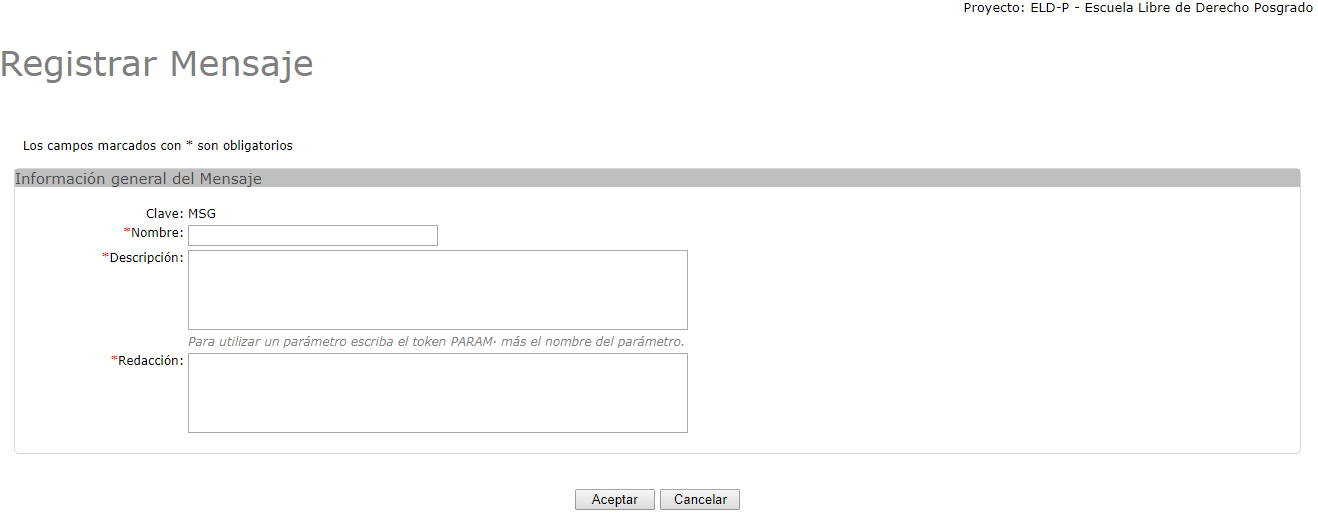
\includegraphics[scale=0.5]{roles/lider/mensajes/pantallas/IU9-1registrarMensaje}
					\caption{Registrar Mensaje}
					\label{fig:registrarMensaje}
				\end{center}
			\end{figure}
		
			\item Ingrese el nombre, una pequeña descripción del mensaje y por último la redacción del mismo. Si es necesario podrá crear un mensaje con parámetros deberá ingresar el token ''PARAM'' e ingresar la descripción del mismo. Así como se muestra en la imagen \ref{fig:registrarMensajeParam}.
			
			\begin{figure}[H]
				\begin{center}
					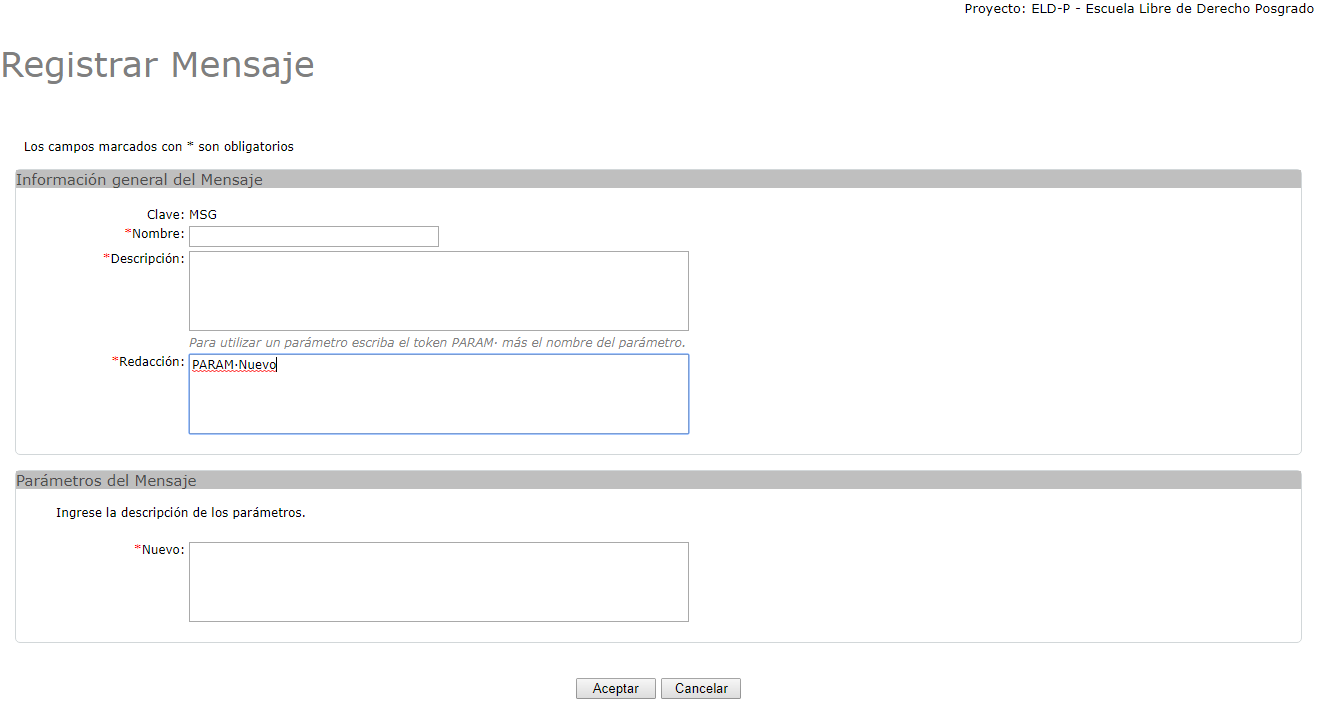
\includegraphics[scale=0.5]{roles/lider/mensajes/pantallas/IU9-1registrarMensajeParam}
					\caption{Registrar Mensaje: Parametrizado}
					\label{fig:registrarMensajeParam}
				\end{center}
			\end{figure}
			
			\item Oprima el botón \IUAceptar.
			
			\item Se mostrará el mensaje \ref{fig:mensajeRegistrado} en la pantalla \ref{fig:GestionarMensajes} ''Gestionar Mensajes''.
			
			\begin{figure}[htbp!]
				\begin{center}
					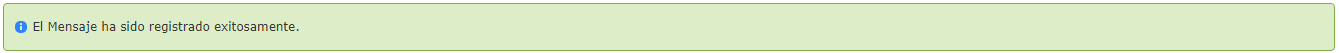
\includegraphics[scale=0.5]{roles/lider/mensajes/pantallas/IU9-1MSG1}
					\caption{MSG: Mensaje Registrado}
					\label{fig:mensajeRegistrado}
				\end{center}
			\end{figure}
			\end{enumerate}